\section{Deterministic model}
\label{sec:model}
We subdivide the classic SIRD compartments, Susceptible ($S$), Infectious ($I$), Recovered ($R$) and Deceased ($D$), with sub-compartments allowing for heterogeneous areas of residence and vaccination states as well as infections by different virus types. Figure \ref{fig:model} illustrates the general model. Individuals either live in country $A$ or country $B$. They are non-vaccinated $U_0$, vaccinated with vaccine one $U_1$ or vaccinated with vaccine two $U_2$. Vaccine $U_1$ represents the messenger ribonucleic acid (mRNA) vaccines and vaccine $U_2$ represent the vector vaccines. We assume that one vaccination shot is sufficient to get full protection of vaccine $U_l$. We introduce two virus types. A wild type $W$ that serves as baseline variant and a more infectious mutant variant $M$.\\
\begin{figure}[h!]
\centering
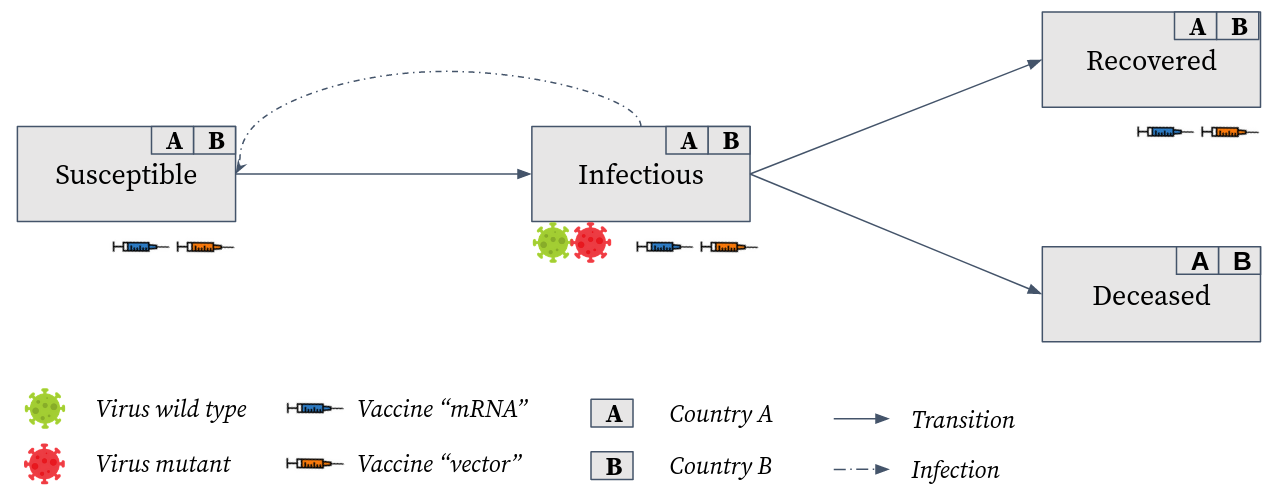
\includegraphics[scale=0.3]{images/vaccination_pp_blue_orange.png}\\
\begin{flushleft}
\scriptsize{\textit{Note}: Solid lines indicate transition paths and dashed lines indicate infections. Shots below a compartment indicate that individuals from this compartment are vaccinated. Viruses below a compartment indicate that this compartment is infectious. Each compartment is subdivided according to country of residence and vaccination status.}
\end{flushleft}
\caption{Model structure}
\label{fig:model}
\end{figure}

To describe our model we denote every sub-group of individuals by a set $\set(F_n)$, where $F_n$ is a placeholder for features that the individuals (elements) within the set $\set$ share and $t$ denotes the time at which the set is evaluated. We illustrate the features $F_n$ in the following with examples. Let $X_i$ for $i \in \{S, I, R, D \}$ indicate to which general compartment an individual belongs, then, $\set(X_S)$ is the set of all susceptible individuals and $\set(X_I)$ is the set of all infectious individuals at $t$. If we want to distinguish not only between general compartments but additionally between countries of residence, we use the feature $C_j$ for $j \in \{A, B\}$ to indicate that the country of residence is $j$. $\set(X_S, C_A)$ is the set of all susceptible individuals of country A and $\set(X_S, C_B)$ of country B. Analogously, $\set(V_k)$ is the set of all individuals infected with virus $k$ and $\set(U_l)$ is the set of all individuals with vaccination status $l$.

We can link sets with the common set operator, e.g. $\set(X_S, C_A) \cup \set(X_S, C_B) = \set(x_S)$ or $\set(X_S) \cap \set(X_I) = \emptyset$. The negation operator $\neg$ is used to indicate that a certain feature applies for all but the specified compartment, e.g. $\set(\neg X_D)$ is the set of all alive individuals. The cardinality $|\cdot|$ represents the respective number of individuals in a set, e.g. $|\set(X_S)|$ equals the number of all susceptible individuals. To shorthand notation, we define $\num(F_n) = |\set(F_n)|$ as the number of individuals within the set $\set(F_n)$. By definition $\set() = \cup_{i \in \{ S, I, R,D\}} \set(X_i)$ is the set of all individuals. An overview of all features is given in Table \ref{tab:features}. \\
\begin{table}[h!]
\centering
\caption{Notation}
\label{tab:features}
\begin{center}
\scalebox{0.8}{
\begin{tabular}{lclp{10cm}}
\hline
\multicolumn{1}{l}{Feature}&\multicolumn{1}{c}{Code}&\multicolumn{1}{c}{Indices}&\multicolumn{1}{c}{Explanation}\\
\hline
\rule{0pt}{2.6ex}General compartment & $X_h$ &  $h \in \{S, I, R, D\}$ & Individuals can either be Susceptible ($S$), Infectious ($I$), Recovered ($R$) or Deceased ($D$). \\
Country of residence & $C_j$ &  $j \in \{A, B\}$ & Individuals can either live in country A or country B.  \\
Virus Type & $V_k$ &  $k \in \{W, M\}$ & An infection can either be caused by the wild type ($W$) or the mutant ($M$) virus. This feature has to be understood, depending on $X_h$, as \textit{is} or \textit{has been} infected with type $k$. For example an individual of $\set(X_I, V_k)$ \textit{is} currently infected and an individual of $\set(X_R, V_k)$ \textit{has been} infected.\\
Vaccine Type & $U_l$ &  $l \in \{0, 1, 2\}$ & An individual can either be vaccinated with vaccine 1 or 2 or being unvaccinated ($U_0$). \\
Placeholder & $F_i$ &  $i \in \mathbb{N}$ & A placeholder that is used to address an arbitrary combination of features. $\set(F_i)$ should be read as the set of a fixed but arbitrary compartment. If we need to distinguish between two arbitrary compartments, we use $F_1$ and $F_2$.\\
\hline
\end{tabular}
}
\end{center}
%\begin{tablenotes}
%\scriptsize
%\item Note: 
%\end{tablenotes}
\end{table}

We impose a set of assumptions to the compartments to rule out undesired cases within the model 
\begin{assumption}\label{ass:model}
For all $t,r \in \R_+$, $k \in \{W,M\}$ and $s \in [-t, \infty)$ let
\begin{align*}
\tag{\ref{ass:model}.1} 
\label{eq:no_reinfections}
\set(X_I, V_k) \cap \mathcal{C}_{t+r}(X_S) &= \emptyset \\
\tag{\ref{ass:model}.2} 
\label{eq:no_double_vaccinations}
\set(U_1) \cap \mathcal{C}_{t+s}(U_2) &= \emptyset \\
\tag{\ref{ass:model}.3} 
\label{eq:no_cross_border_mobility}
\set(C_A) \cap \mathcal{C}_{t+s}(C_B) &= \emptyset  \\
\set(X_S, V_k) &= \emptyset
\tag{\ref{ass:model}.4}.
\label{eq:no_susceptible_infections}
\end{align*}
\end{assumption}
\noindent Assumption \ref{eq:no_reinfections} rules out reinfections such that an individual that has been infected once cannot become reinfected after it had recovered. According to \cite{Roy.2020}, there is evidence that recovered individuals cannot become reinfected but reinfections cannot be ruled out fully. However, the number of reinfected individuals might be negligible and we therefore do not incorporate reinfections to keep our model parsimonious. Assumption \ref{eq:no_double_vaccinations} implies that an individual only receives one type of vaccine. Receiving one vaccination shot in our model implies that an individual is fully protected according to the vaccine properties making it needless to assign a second shot to the same individual. Assumption \ref{eq:no_cross_border_mobility} rules out permanent cross-country movements of individuals. We do so since  permanent movements should not be a main driver of the pandemic and we therefore refrain from incorporating it to keep our model parsimonious. We incorporate cross-border infections by assigning a fraction of infections to be a cross-border infections.
Assumption \ref{eq:no_susceptible_infections} ensures that susceptible individuals cannot be associated with any type of virus, since they have not been infected yet and can become infected with both virus types.

\subsection{System of ordinary differential equations}
We use a compartment SIRD model, based on a system of ordinary differential equations (ODEs), to simulate the pandemic. We see every subcompartment as own chemical species and each transmission, e.g. vaccinations, infections, recoveries, and deaths, as chemical reaction. Thus, our system becomes a chemical reaction network. To make this thesis self-contained, we explain how the dynamics of a chemical reaction network are modeled using ODEs. We can limit ourselves to the case of irreversible reactions since recovered and deceased individuals cannot become infectious again and infectious individuals become recovered but not susceptible. \\

Let $\set(F_1), \dots, \set(F_n)$ be $n$ pairwise disjoint sets and $\cup_{i=1}^n \set(F_i) = \set()$. Every irreversible reaction $R_j$, for $j = 1, \dots, m$, can be expressed as reaction of all compartments
\begin{align}
\underbrace{\nu_{1j} \num(F_1) + \hdots + \nu_{nj} \num(F_n)}_{Reactants} \longrightarrow \underbrace{\mu_{1j} \num(F_1) + \hdots + \mu_{nj} \num(F_n)}_{Products},
\end{align}
where $\nu_{ij} \in \mathbb{N}_0$ and $\mu_{ij} \in \mathbb{N}_0$ are called stoichiometric coefficients.  If a compartment $\set(F_i)$ is not a reactant or product within reaction ,$R_j$ the respective stoichiometric coefficients $\nu_{ij}, \mu_{ij}$ are set to zero. $\nu_{ij}$ describes how much of species $\set(F_i)$ is consumed and $\mu_{ij}$ how much is produced within reaction $R_j$. The difference $\mu_{ij} - \nu_{ij}$ is the total change of $\num(F_i)$ due to one reaction $R_j$.

We are not only interested in how one reaction (e.g. an infection, a vaccination, etc.) influences the state of the system but rather how often this happens within an interval $[t, t+\tau]$, for $\tau \in \R_+$. If we restrict us to the case $\tau = 1$, the latter is described according to the law of mass action by
\begin{align}
\label{eq:change_one_unit}
v_j = r_j  \prod_{i=1}^n \num(F_i)^{\mu_{ij}},
\end{align}
where $r_j$ is a reaction specific constant. The product is the number of combinations to assign individuals from different compartments, that have $\mu_{ij} \neq 0$, together.

The change in the magnitude of $\num(F_i)$ within the interval $[t, t+\tau]$ is given by the sum of the influences of all $m$ reactions
\begin{align}
\label{eq:sys_change}
y_{t+\tau}(F_i) - \num(F_i) = \sum_{j=1}^m (\mu_{ij} - \nu_{ij}) v_j \tau.
\end{align}
$(\mu_{ij} - \nu_{ij})$ is, as outlined above, the stoichiometry that specifies how one reaction influences the system, $v_j \tau$ is the number of times reaction $R_j$ happens within the interval $[t, t+\tau]$, and therefore the product is the influence of $R_j$ on $\num(F_i)$ within $[t, t+\tau]$. Summed over all reactions yields the change of $\num(F_i)$ within the system. 

We divide both sides of \eqref{eq:sys_change} by $\tau$, let $\tau \to 0$ and plug in \eqref{eq:change_one_unit} to obtain the ordinary differential equation
\begin{align}
\der(F_i) = \sum_{j=1}^m \left[(\mu_{ij} - \nu_{ij}) r_j  \prod_{i=1}^n \num(F_i)^{\mu_{ij}} \right].
\end{align}
We write down the equations for all compartments in matrix form to obtain the system of ODEs, which we use in subsequent chapters to ease notation.
\begin{align}
\label{eq:ode_system_matrix}
\underbrace{\begin{pmatrix}
\der(F_1) \\ \vdots \\ \der(F_n) \end{pmatrix}}_{Y(t)} =
\underbrace{\begin{pmatrix}
\mu_{11} - \nu_{11} & \hdots & \mu_{1m} - \nu_{1m} \\
\vdots & \vdots & \vdots \\
\mu_{n1} - \nu_{n1} & \hdots & \mu_{nm} - \nu_{nm} \\
\end{pmatrix}}_{\vect{S}} \cdot
\underbrace{\begin{pmatrix}
v_1 \\ \vdots \\ v_m
\end{pmatrix}}_{v}
\end{align}
%For ODE system's it is common to elaborate on the steady-state of the system. Note that \eqref{eq:ode_system_matrix} is a linear mapping in $v$ for which we can compute the kernel $\mathcal{K}=\left\{v \in \R^m | \vect{S} \cdot v = 0 \in \R^n  \right\}$. Each element of the kernel represents a state where $Y(t)=0$ and therefore the system is in a steady- state. If the pandemic reaches a state such that $v \in \mathcal{K}$, we would be stuck there.  \\

Since our model consists of over 100 reactions, we do not write down the ODE system explicitly. However, it can be constructed as stated within this section.  
\subsection{Reactions}
From a chemical point of view, our model can be divided into four major groups of reactions: 1. Infections, 2. Recoveries and Deaths and 3. Vaccinations. We group recoveries and deaths together, since their reactions have the same structure. We subsequently state the general and explicit reactions. We define the reactants, products, stoichiometric coefficients and reaction constants, such that that the ODE system \eqref{eq:ode_system_matrix} is determined. We emphasize reaction constants since they incorporate most information, such as vaccination status and infectiousness of the virus, of our model.


\subsubsection{Infections}
\begin{figure}[h!]
\centering
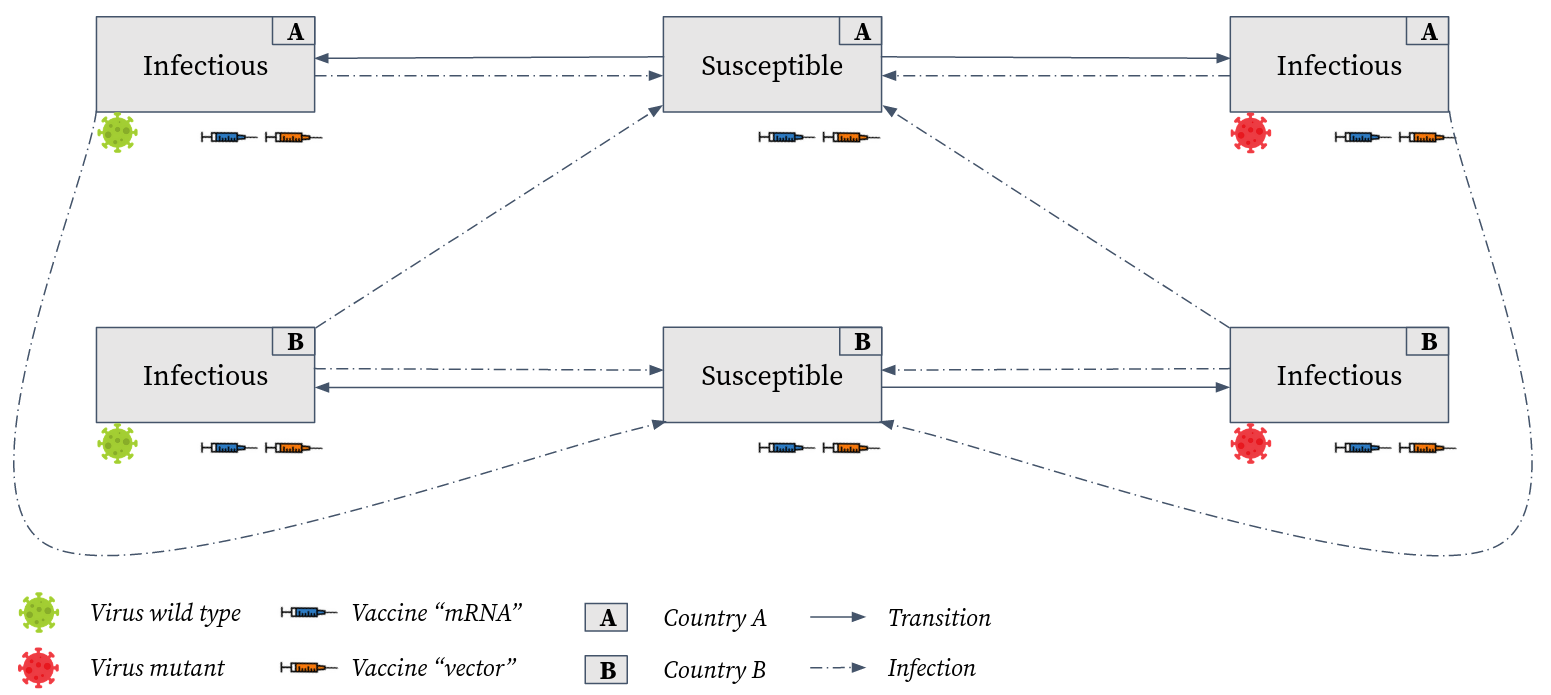
\includegraphics[scale=0.3]{images/overview_infection.png}\\
\begin{flushleft}
\scriptsize{\textit{Note}: Solid lines indicate transition paths and dashed lines indicate infections. Shots below a compartment indicate that individuals from this compartment can be vaccinated. Viruses below a compartment indicate that this compartment is infectious with the respective virus type. The letters in the top right corner of each compartment indicate the country of residence of individuals within the compartment.}
\end{flushleft}
\caption{Infection structure}
\label{fig:model_infections}
\end{figure}
Figure \ref{fig:model_infections} depicts the structure of the transmissions from the susceptible to the infectious compartments. Every infectious individuals $i_1 \in \set(x_I)$ can infect a susceptible individual $i_2 \in \set(x_S)$ regardless of their countries of residence. However, we account for the higher chance of becoming infected due to an individual from the same country by shrinking the influence of the infectious compartments from the respective other country via the reaction constants. \\

In chemical terms, the compartments of two individuals $i_1$ and $i_2$ serve as reactants and their compartments with $i_2$ infected as products yielding the general form of the infection reactions
\begin{align}
\label{eq:general_infection}
\num(x_I, F_1) + \num(x_S, F_2) \longrightarrow \num(X_I, F_1) + \num(X_I, F_2),
\end{align}
where we use $F_1, F_2$ to indicate that the reactions differ with respect to not explicitly mentioned features, e.g. vaccinated individuals have a lower risk of becoming infected or transmitting the virus, the mutant virus is more infectious, and cross-border infections are scaled by a factor to make them comparatively rare events. If $F_1 \neq F_2$, the stoichiometric coefficients are one. If $F_1=F_2$, they are one for the reactants but two for the products while only having one product. We incorporate the additional features, represented by $F_1$ and $F_2$, within the reaction constants, which we label as \textit{infection constants}
\begin{align*}
\text{infection constant} = \text{infections per day} \times \text{vaccine modifier} \times \text{compartment adjustment}
\end{align*}
In the following, we elaborate on how to define the components of the \textit{infections per day}, the \textit{vaccine modifiers}, and the \text{compartment adjustments}.\\

\textbf{Infections per day.} To compute the infections per day we use the average number of contacts, between infectious and susceptible individuals, and multiply it with the proportion of individuals that become infected while meeting an infectious individual.

Let $c \in R_+$ be the average number of contacts per individual and day and $\alpha \in [0,1]$ be the proportion of susceptible individuals that become infected if they meet a wild type infected individual without any vaccination of both individuals. Let $\eta \in (1, 1/\alpha]$ be the factor with which the mutant is more infectious than the wild type. Then $\beta = \alpha c$ is the average number of individuals infected per day by $i_1$ if $i_1 \in \set(X_I, V_w, U_0)$. If $i_1 \in \set(X_I, V_M, U_0)$ the average infected number increases to $\eta \beta$. We label $\beta$ as \textit{baseline infection constant}, since it covers the most basic case where the reaction happens between an unvaccinated susceptible individual and an unvaccinated wild type infected individual. \\

\textbf{Vaccine modifier.} Vaccinations influence the infections via two channels. First, vaccinated susceptible individuals are less likely to become infected, see Table \ref{tab:efficacy} for a list references. Second, vaccinated infectious individuals are less likely to transmit the virus \citep{Harris.2021}.

To account for the influence of the first channel, we introduce the parameters $\delta_{k,l} \in [0,1]$, where $k \in \{W, M\}$ indicates the virus type and $l \in \{ 1,2\}$ the vaccine type. $\delta_{k,l}$ is the reduce in the probability of becoming infected while meeting an infectious individual after being vaccinated. Thus, susceptible individuals are $1 - \delta_{k,l}$ times less likely to become infected while meeting an infectious individual. This is incorporated within the infection constant by multiplying the baseline infection constant with $1 - \delta_{k,l}$ if $i_s \in \set(X_S, U_1) \cup \set(X_I, U_2)$.

We account for the second channel two by introducing the parameter $\gamma \in [0,1]$. $\gamma$ is the reduction in the probability of not transmitting the virus after being vaccinated, which we assume to be constant over time and across vaccines. Analogously to the first channel, we  multiply the baseline infection constant with $(1 - \gamma)$ if $i_1 \in \set(X_I, U_1) \cup \set(X_I, U_2)$.  \\

\textbf{Compartment adjustments.} So far we have only defined the average number of contacts per day $c$ of an infectious individual $i_1 \in \set(X_I, F_1)$ but not specified how these contacts are distributed across compartments. We use $\prob_t(i_2 \in \set(X_S, C_j, F_2) | i_1 \in \set(X_I, F_1))$, the conditional probability that the second individual $i_2$ is susceptible and from compartment $\set(X_S, C_j, F_2)$, and multiply it by $\beta$ to get baseline infection constant adjusted by the average number of contacts between $i_1$ and individuals of the compartment $\set(X_S, F_2)$. Note that the probability $\prob_t$ depends on the state of the whole system $Y(t)$. To increase readability we omit conditioning on $Y(t)$ and directly define $\prob_t$ to be conditioned on the state of the system $Y(t)$.

We assume that the vaccination status, the type of virus infection, and the exact general compartment ($X_S, X_I, X_R$) of $i_1$, are independent of $\prob_t(i_2 \in \set(X_S, C_j, F_2)) $. Thus, the problem facilitates to finding $\prob_t(i_2 \in \set(X_S, F_2) | i_1 \in \set(\neg X_D, C_{j'}))$. This to say, the probability that the individual that can be infected ($i_2$) is susceptible, unvaccinated and from area two given that individual $i_1$ is infected with the wild type, unvaccinated and from area one. We facilitate our model and assume that the vaccination status as well as the type of virus infection of individual $i_1$ are independent of the features of $i_2$. Assuming independence of the vaccination status implies that an unvaccinated individual $i_1$ does not change her contact habits, given a certain number of meetings, compared to her counterfactual vaccinated self. Note that this does not mean that we assume that vaccinated and unvaccinated individuals have the same average number of contacts since the probabilities are defined on \textit{conditioned a meeting occurs}. Differences in the average number of contacts between vaccinated and unvaccinated individuals can be incorporated implicitly via the vaccination parameter $\delta_{k,l}$.

To facilitate notation we subsequently take the perspective that the infectious individual lives in country A. The same math applies vice versa. We provide a detailed derivation of the probabilities within the Appendix \ref{A:meeting_prob}.
\begin{align}
\label{eq:cond_meeting_prob}
\prob_t(i_2 \in \set(X_S, C_j, F_2)|i_1 \in \set(\neg X_D, C_A)) &= \begin{cases} 
      1-\frac{\num(X_S, C_j, F_2)}{\num(\neg X_D)} \cdot b(d(A, B)), & j = A \\
      \frac{\num(X_S, C_j, F_2)}{\num(\neg X_D)} \cdot b(d(A, B)), & j = B 
   \end{cases}
\end{align}
The probability is in essence the relative population size adjusted for lower cross-border meeting frequencies by a penalty function $b: \R_+ \to [0,1]$ that depends on the distances between both countries $d(A, B)$. By mapping the distance into the unit interval, we allow the probability of a cross-border meeting to be maximal as high as the relative population size. The distance can be interpreted as geographical distance but it could also serve to incorporate other factors, like favored holiday destinations, that encourage or discourage cross-border meetings. We impose three conditions on the function $b$
\begin{align}
\lim_{b \to \infty} &= 0 \tag{B.1}\\
b(0) &= 1 \tag{B.2}\\
b(d_1) &< b(d_2) \quad \textrm{if } d_1 > d_2. \tag{B.3}
\end{align}
Condition $(B.1)$ ensures that countries that a very large distance only have small influences onto each other, $(B.2)$ defines a rather theoretical case where cross-border meetings are as likely as within-country meetings, and $(B.3)$ ensures that countries that have a greater distance have a smaller influence onto each other. \\

\textbf{Explicit reactions.}
With the derived specifications of the infections per day, the vaccine modifiers, and the compartment adjustments, we are able to specify the compartment specific infection constants. We illustrate this by two examples. 

\begin{example}
Let the reactants be the compartments $\set(X_{I}, C_A, V_W, U_0)$ and $\set(X_{S}, C_B, U_0)$. The corresponding reaction is
\begin{align}
\num(X_{I}, C_A, V_W, U_0) + \num(X_{S}, C_B, U_0) &\xrightarrow{ r_{j_1}} \num(X_{I}, C_A, V_W, U_0) + \num(X_{I}, C_B, V_W, U_0),
\end{align}
where $r_{j_1}$ denotes the infection rate. To account for the infections per day, we use the baseline infection constant $\beta$, since the infectious compartment is infected with the wild type. The susceptible and the infectious compartments are unvaccinated. We therefore do not multiply by a vaccine modifier. However, the compartments are from different countries. We therefore adjust by multiplying with $\frac{\num(X_S, C_j, F_2)}{\num(\neg X_D)} \cdot b(d(A, B))$
\begin{align}
r_{j_1} = \beta \cdot \frac{\num(X_S, C_j, F_2)}{\num(\neg X_D)} \cdot b(d(A, B))
\end{align}
\end{example}

\begin{example}
For the second example, we consider vaccinated and mutant infected compartments $\set(X_{I}, C_A, V_M, U_1)$ and $\set(X_{S}, C_B, U_2)$ as reactants to showcase the influence of the vaccine and the mutant modifier. 
\begin{align}
\num(X_{I}, C_A, V_M, U_1) + \num(X_{S}, C_B, U_2) &\xrightarrow{ r_{j_2}} \num(X_{I}, C_A, V_M, U_1) + \num(X_{I}, C_B, V_M, U_2).
\end{align}

Since the infectious individual is infected with the mutant, we multiply the baseline infection constant with $\eta$. Since the infectious compartment is vaccinated, we multiply the constant with $(1-\gamma)$. Since the susceptible compartment is vaccinated with vaccine $U_2$, we multiply the infection constant with $1-\delta_M,2$. The compartments are from different countries. We therefore adjust by multiplying with $\frac{\num(X_S, C_j, F_2)}{\num(\neg X_D)} \cdot b(d(A, B))$
\begin{align}
r_{j_2} = (1-\delta_{M,2}) (1-\gamma) \eta \beta  \frac{\num(X_S, C_j, F_2)}{\num(\neg X_D)} \cdot b(d(A, B)).
\end{align}
\end{example}

To ensure readability we refrain from writing down all exact infections but they can be derived as shown in the two examples.

\subsubsection{Recoveries and deaths}
\begin{figure}[h!]
\centering
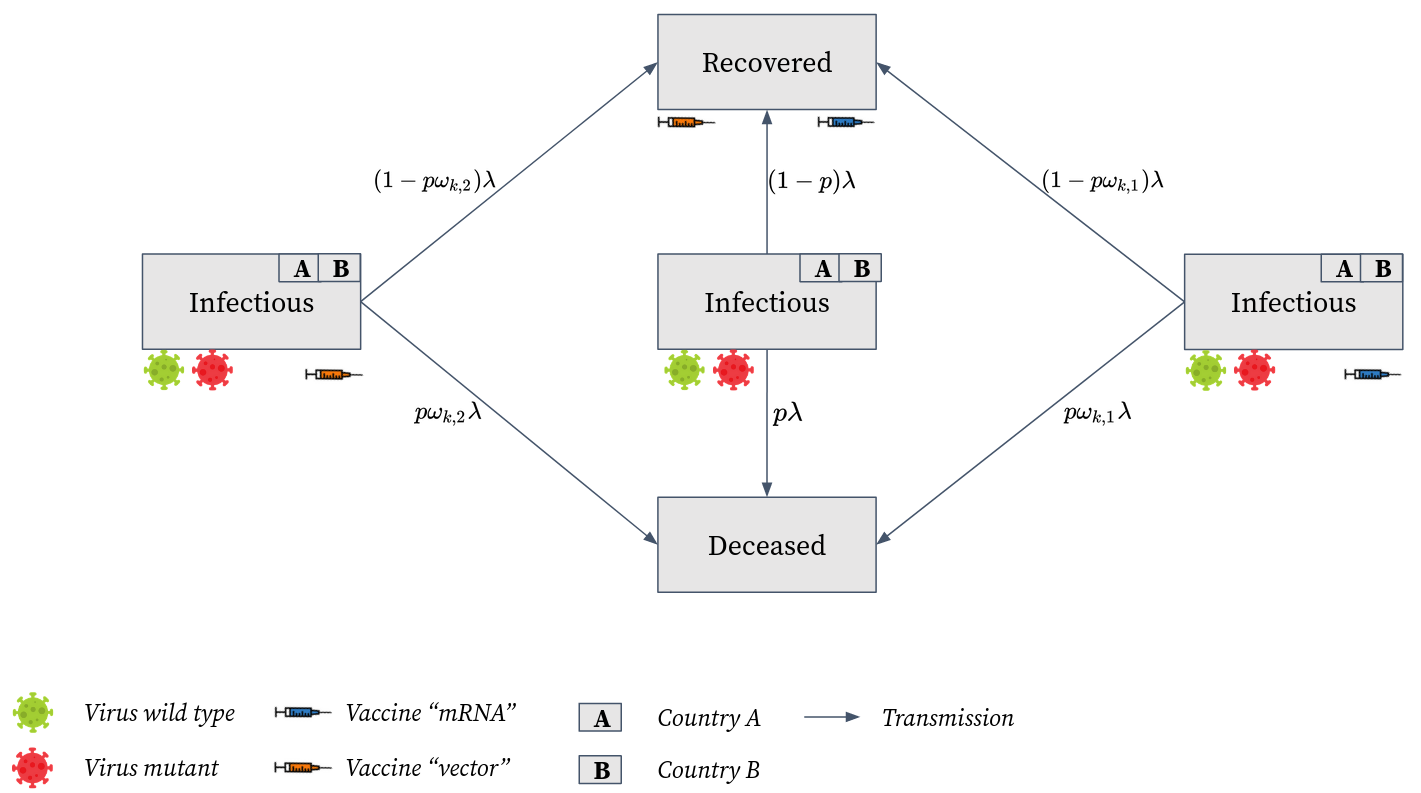
\includegraphics[scale=0.3]{images/overview_recovery.png}\\
\begin{flushleft}
\scriptsize{\textit{Note}: Solid lines indicate transition paths. Shots below a compartment indicate that individuals from this compartment are vaccinated. Viruses below a compartment indicate that this compartment is infectious with the respective virus type. The letters in the top right corner of each compartment indicate the country of residence of individuals within the compartment. The formulas on top of the solid lines indicate the respective reaction constant.}
\end{flushleft}
\caption{Structure of recoveries and deaths}
\label{fig:model_recoveries}
\end{figure}
Figure \ref{fig:model_recoveries} depicts the dynamics of the recoveries and deaths. The general reactions are defined by one infectious reactant and one product
\begin{align}
\label{eq:recovery}
    \set(X_I, F_1) & \longrightarrow  \set(X_D, F_1) \\
    \set(X_I, F_1) & \longrightarrow  \set(X_R, F_1). \notag
\end{align}
The reaction number is the product of the average number of individuals transmitting out of the reactant compartment $\set(X_I, F_1)$ and the fraction of individuals that transmit to the product compartment, either $\set(X_D, F_1)$ or $\set(X_R, F_1)$. \\

Let $\lambda \in \R_+$ be the average number of individuals that transmit out of $\set(X_I, F_1)$. We assume that a constant fraction $p \in [0,1]$ of these individuals dies. Hence, $p\lambda$ individuals transmit to the deceased and $(1-p)\lambda$ individuals transmit to the recovered state. 
The explicit reactions for unvaccinated individuals are for $i \in \{A, B\}$ and $k \in \{W, M\}$
\begin{align}
    \set(X_I, C_j, V_W, U_0) &\xrightarrow{p \lambda} \set(X_D,C_j, V_w, U_0)  \\
    \set(X_I, C_j, V_w, U_0) &\xrightarrow{(1-p) \lambda} \set(X_R,C_j, V_w, U_0) \notag
\end{align}
$1/\lambda$ is the average durationan individual spends within $\set(X_I, F_1)$. We have implicitly assumed that this time is the same for deceasing and recovering individuals, which might not be accurate in real-world examples since deceasing individuals have more severe cases and heavier viral loads, such that they stay longer infectious. However, incorporating the seperated average duration would raise the need for more compartments. Since we allow for vaccinations of recovered and infectious individuals, we assume that this simplification is negligible. Moreover, note that $p$ does not depend on the virus type. The virus type therefore only influences the number of infections but not the probability of dying for infected individuals. According to \cite{Davies.2021} this assumption might be violated. We do so however, since we difference is rather low and we want to keep our model simple. \\


If the infectious individuals are vaccinated, they are less likely to decease \citep{Tenforde.2021, Voysey.2021}. To account for this reduce in the fraction that transmits to the deceased state, we introduce the parameters $\omega_{k,l} \in [0,1]$, for $k \in \{W, M\}$ and $l \in \{1,2\}$. We use $p \omega_{k,l}$ as new probability of dying due to being infected with virus $k$ after being vaccinated with vaccine $l$. $\omega_{k,l}$ is thus the reduction in the probability of dying. The corresponding reactions for vaccinated individuals are for $i \in \{A, B\}, k \in \{W, M\}$ and $l \in \{1,2\}$
\begin{align}
    \set(X_I, C_j, V_k, U_l) &\xrightarrow{p \omega_{k,l} \lambda} \set(X_D,C_j, V_k, U_l) \\
    \set(X_I, C_j, V_k, U_l) &\xrightarrow{(1-p \omega_{k,l}) \lambda} \set(X_R,C_j, V_k, U_l) \notag
\end{align}

\subsubsection{Vaccination}
\begin{figure}[h!]
\centering
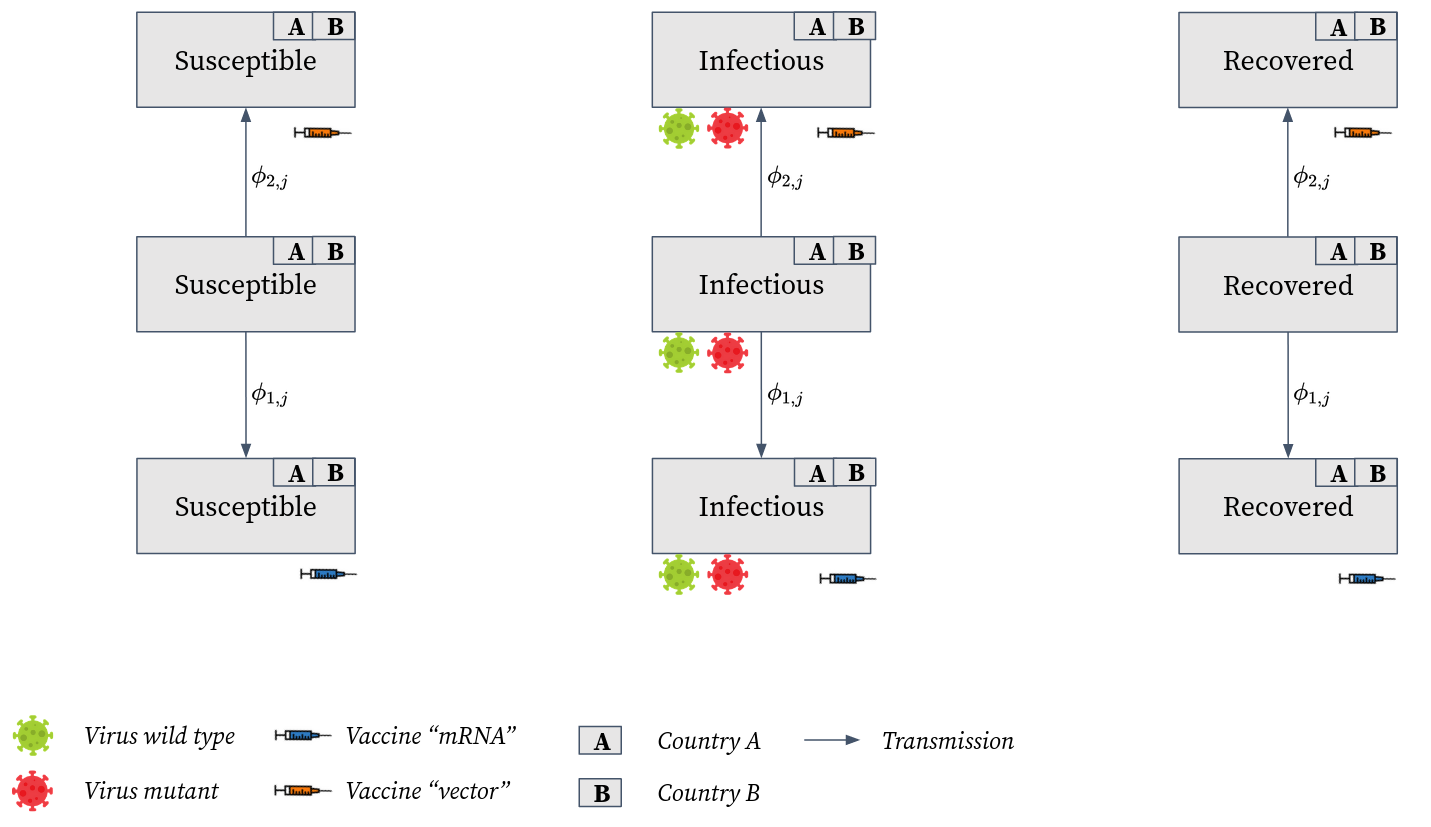
\includegraphics[scale=0.3]{images/overview_vaccination.png}\\
\begin{flushleft}
\scriptsize{\textit{Note}: Solid lines indicate transition paths. Shots below a compartment indicate that individuals from this compartment are vaccinated with the respective vaccine. Viruses below a compartment indicate that this compartment is infectious. The letters in the top right corner of each compartment indicate the country of residence of individuals within the compartment. The formulas next to the solid lines indicate the respective reaction constant.}
\end{flushleft}
\caption{Structure of vaccinations}
\label{fig:model_vaccination_ov}
\end{figure}
Figure \ref{fig:model_vaccination_ov} depicts the vaccination dynamics. We allow for vaccinations of susceptible, recovered and, deceased individuals. We vaccinate susceptible individuals since these individuals to protect them from becoming infected. We vaccinate nfectious individuals to account for asymptomatic cases \citep{Byambasuren.2020} and recovered individuals to account to increase their degree of immunity \citep{Skelly.2021}. \\

Let $\phi_{l,j} \in \R_+$ be the vaccination constant of vaccine $l$ in country $j$ at time $t$. The vaccination constant of one vaccine is assumed to be equal for all vaccination subcompartments of $S, I,R$ within one country, which is to say, that the decision of vaccinating an individual is independent whether it is susceptible, infectious or recovered.  The corresponding reactions are for $j \in \{A,B\}$, $k \in \{W,M\}$ and $l \in \{1,2\}$
\begin{align}
\set(X_S, C_j, U_0) &\xrightarrow{\phi_{l, j}} \set(X_S, C_j, U_l)  \\
\set(X_I, C_j, V_k, U_0) &\xrightarrow{\phi_{l,j}} \set(X_I, C_j, V_k, U_l) \notag \\
\set(X_R, C_j, V_k, U_0) &\xrightarrow{\phi_{l,j}} \set(X_R, C_j, V_k, U_l). \notag
\end{align}
The vaccination constant is determined by the implemented vaccination policy. We explain how the vaccination constant is derived, given a vaccination policy, in Chapter \ref{sec:vaccine_allocation}.


